\documentclass[journal]{IEEEtran}
\usepackage{graphicx}
\usepackage{float}
\author{MQuang-Cuong Pham and Yoshihiko Nakamura
\\Department of Mechano-Informatics
\\University of Tokyo, Japan}
\title{\textbf{Time-Optimal Path Parameterization for Critically Dynamic Motions of Humanoid Robots}}

\begin{document} 

\maketitle

\begin{abstract}
Planning collision-free, dynamically-balanced movements for humanoid robots is a challenging problem. An effective approach consists of first planning a motion satisfying geometric and kinematic constraints (such as collision avoidance, joint angle limits, velocity limits, etc.) and, in a second stage, modifying this motion so that it respects dynamic balance criteria, such as those relative to the Zero Moment Point (ZMP). However, this approach currently suffers from the issue that the modified motion may give rise to new collisions with respect to the original motion, which can be very costly to deal with, especially for systems with many degrees of freedom and cluttered environments. Here we present an algorithm to modify the motions of humanoid robots under ZMP constraints without changing the original motion path, making thereby new collision checks unnecessary. We do so by adapting the minimum-time path parameterization under torque constraints algorithm of Bobrow et al. to the case of ZMP constraints. In contrast with a previous approach based on finite differences and iterative optimization to find the optimal path parameterization under ZMP constraints, our Bobrow-based algorithm finds this optimal parameterization in a single pass. We demonstrate the efficiency of this algorithm by simulations.
\end{abstract}

\section{INTRODUCTION}
Planning collision-free, dynamically-balanced movements
for humanoid robots is a challenging problem because of the robots’ large numbers of degrees of freedom and the issue of balance inherently associated with the erect posture.

An effective approach consists of first generate robot
motions that satisfy geometric and kinematic constraints,
such as collision avoidance, joint angle limits, velocity limits, satisfaction of high-level tasks, etc. Many powerful and versatile algorithms (which can also be combined with each other) allow to do so, just to name a few: prioritized inverse kinematics with equality and inequality constraints (see e.g. [19, 5]), randomized motion planning (see e.g. [6, 20]), motion retargeting from captured data (see e.g. [3, 7]), etc.

To take into account the standing/walking balance issues,
these approaches typically involve the further condition that the projection of the Center of Mass (CoM) on the ground stays within the convex hull of the ground contact points – which can indeed be expressed as a purely geometric constraint. However, this condition on the CoM effectively guarantees robot balance only when the robot is assumed to move quasi-statically, that is, with a close-to-zero speed. If the motion speed is non-negligible, the CoM condition is inoperative: there exist motions that satisfy the CoM con-dition without being dynamically balanced and, conversely, there exist motions that are dynamically balanced without satisfying the CoM condition. A much appropriate condition for dynamic balance is that the Zero Moment Point (ZMP) should stay in the convex hull of the ground contact points (cf. [17])

It is thus necessary, in a second step, to modify the motions
computed by the previously mentioned algorithms to make
them satisfy the condition for dynamic balance expressed
by the ZMP. There are basically two methods to do so:
the first method consists of scaling down the motion speed,
such that the motion is executed in a quasi-static manner
(cf. [6]). This method has the obvious drawback that it
may generate very slow movements. The second method
consists of “filtering” a non-dynamically-balanced motion
into a dynamically-balanced one considering the whole-body
dynamics (see e.g. the balance compensation algorithm [4]
or the “dynamics filter” algorithm [18]). However, these
algorithms suffer from a serious issue: they modify the
motion path, such that the “filtered” motion may give rise to
new collisions with respect to the original motion. Therefore,
these algorithms must check collisions again at each time
step, which can be very costly, especially when the robot
has many degrees of freedom or when the environment is
cluttered. In fact, it is well known that dealing with collisions
in such cases takes the biggest part of the computation time
during the kinematic planning step.

Here we modify the motion by time-reparameterizing it:
the original motion path remains thus unchanged, making
new collision checks unnecessary. In contrast with the “scal-
ing down” method previously discussed, the motions retimed
by this method are not necessarily quasi-static, and can
indeed be sometimes even faster than the original motions.
This method is based on an algorithm first developed by
Bobrow and other researchers in the 80’s and 90’s, which
allows efficiently finding a time-parameterization of a given
motion path that minimizes the execution time while respect-
ing actuator torque limits [1, 12, 13, 11] (from now on,
we shall refer to this algorithm as the “Bobrow algorithm”
for convenience, but in no way we are underestimating the
essential contributions of the other researchers). The key of
the present article is thus to express the ZMP constraints
in a form compatible with the Bobrow algorithm. Fig. 1
summarizes our approach.

The idea of using path reparameterization to handle ZMP
constraints has been previously proposed by Suleiman et

\begin{figure}
  \centering
  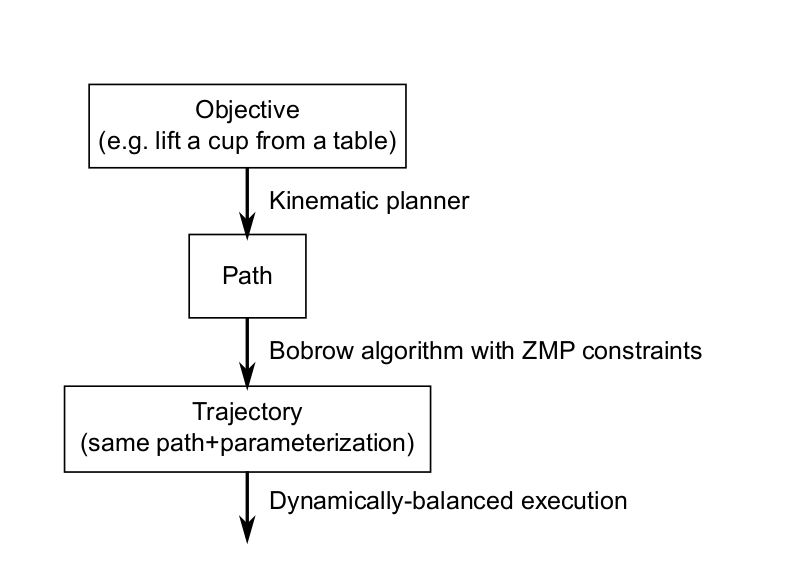
\includegraphics[width=.4\textwidth]{1.png}
  \caption{Sketch of the “two-steps” approach.}
  \label{img1}
\end{figure}

al. [15]. While aware of the Bobrow algorithm, the authors
thought it would be difficult to apply it to the case of
humanoid robots. Instead, they followed an iterative opti-
mization approach by considering a basis of the solution
space (the space of the path parameterization functions s,
cf. section II) and by optimizing the coefficients multiplying
the basis functions. This approach thus usually yields a
very large optimization problem: for instance, to obtain a
satisfactory result in a whole-body reaching tasks, the authors
needed to consider an optimization in 120 variables, which
took 27 iterations to converge (and it was unclear whether
the true optimum had been reached). Here we show that
it is possible to apply the Bobrow algorithm to the case
of humanoid robots and that, following this approach, the
true optimal, critical (because the ZMP is always on the
border of the authorized area, in contrast with [15] and in
accordance with the theory of time-optimal control [1, 13]),
path parameterization can be found in a single pass.

Note that, rather than following a “two-steps” approach
as discussed so far, some methods take into account the
ZMP constraint directly at the planning stage, by consid-
ering either a simplified inverted pendulum model of the
robot (see e.g. [14] and references therein) or the robot
whole-body dynamics (see e.g. [8] and references therein).
While inverted-pendulum-based methods are appropriate to
generate online walking motion, they are not suited for more
complex behaviors involving for instance hierarchies of tasks.
On the other hand, planning methods that take into account
whole-body dynamics still lack the robustness and versatility
of kinematics planning methods.

The rest of the article is organized as follows. In sec-
tion II we show how to express the ZMP constraints in a
form compatible with the Bobrow algorithm and discuss the
specificities of these constraints. In section III, we show some
simulation and experimental results on a humanoid robot.
Finally, in section IV, we briefly discuss the advantages and
limitations of the proposed approach, as well as its possible
future developments.

\section{MINIMUM - TIME PATH PARAMETERIZATION ALGORITHM}
\subsection{Reducing the ZMP equations to the “Bobrow form”}
Consider a legged robot composed of interconnected rigid
links. A well-known condition for the robot dynamic balance
is that the ZMP stays within the convex hull of the ground
contact points at any time instant [17]. The X-coordinate of the ZMP is given by
$$
x_{\textbf{ZMP}}=\frac{\sum_{i}m_{i}(\ddot{z}_{i}+g)x_{i}-\sum_{i}m_{i}\ddot{x}_{i}z_{i}-\sum_{i}(\textbf{M}_{i})_{y}}{\sum_{i}m_{i}(\ddot{z}_{i}+g)}
$$
where $x_{i}$, $y_{i}$, $z_{i}$ are the coordinates of link $i$, $\omega_{i}$ its angular
velocity, $m_{i}$ its mass, $\textbf{I}_{i}$ its inertia matrix and $\textbf{M}_{i} = \textbf{I}_{i}\dot{\omega}_{i} + \omega_{i} \times \textbf{I}_{i}\omega_{i}$. The Y-coordinate of the ZMP can be computed by a similar formula [9].

Next, by forward kinematics, one can express $\textbf{p}_{i}=(x_{i} , y_{i} , z_{i})$ as a nonlinear function of the generalized coordi- nates \textbf{q} (typically, \textbf{q} may contain the translation and rotation of the base-link together with the joint angles)
$$
\textbf{p}_{i}=\textbf{r}^{p}(\textbf{q})
$$
Successively differentiating the above relation yields (drop-ping the argument q for simplicity)
\begin{equation}
\dot{\textbf{p}}_{i}=\textbf{r}^{p}_{\textbf{q}}\dot{\textbf{q}}
\end{equation}
and
\begin{equation}
\ddot{\textbf{p}}_{i}=\textbf{r}^{p}_{\textbf{q}}\ddot{\textbf{q}}+\dot{\textbf{q}}^{\top}\textbf{r}^{p}_{\textbf{qq}}\dot{\textbf{q}},
\end{equation}
where $\textbf{r}^{p}_{\textbf{q}}$ and $\textbf{r}^{p}_{\textbf{qq}}$ are respectively the Jacobian matrix (of
dimension $3\times n$, where n is the dimension of \textbf{q}) and the Hessian tensor (of dimension $3\times n\times n$) of $\textbf{r}^{p}$ with respect to \textbf{q}.

Assume that we are given a twice-differentiable motion
trajectory $\textbf{q}(t)_{t\in[0,T]}$. We say that s is a path \emph{parameter-ization function} if it is an increasing, twice-differentiable function $s : [0, T'] → [0, T ]$. Next, q can be expressed as a
function of the path parameter $s$ as $\textbf{q} = \textbf{q}(s)$, which in turn yields
\begin{equation}
\dot{\textbf{q}}=\textbf{q}_{s}\dot{s}
\end{equation}
and
\begin{equation}
\ddot{\textbf{q}}_{i}=\textbf{q}_{s}\ddot{s}+\textbf{q}_{ss}\dot{s}^{2}
\end{equation}

Substituting (3) and (4) in (2) yields
$$
\ddot{\textbf{p}}_{i}=(\textbf{r}^{p}_{\textbf{q}}\textbf{q}_{ss}+\textbf{q}^{\top}_{s}\textbf{r}^{p}_{\textbf{qq}}\textbf{q}_{s})\dot{s}^{2}
$$
The above equation implies that ẍ i can be expressed as a
function of $s,\dot{s}^{2},\ddot{s}$ as follows
$$
\ddot{x}_{i}=a_{x_{i}}(s)\ddot{s}+b_{x_{i}}(s)\dot{s}^{2},
$$
and similarly, $\ddot{y}_{i},\ddot{z}_{i}$ can be expressed as functions of $s,\dot{s}^{2},\ddot{s}$.

Turning to the term in ω i in the expresion of $x_{\textbf{ZMP}}$, remark that one can write
$$
\omega_{i}=\textbf{r}^{\omega}(\textbf{q})\dot{\textbf{q}},
$$
where $\textbf{r}^{\omega}$ is a $3 \times n$ matrix. Thus, one has (dropping the argument q for simplicity)
$$
\dot{\omega_{i}}=\textbf{r}^{\omega}\ddot{\textbf{q}}+\dot{q}^{\top}\textbf{r}^{\omega}_{\textbf{q}}\dot{\textbf{q}},
$$
where $\textbf{r}^{\omega}_{\textbf{q}}$ is the Jacobian tensor (of dimension $3 \times n\times n$) of $\textbf{r}^{\omega}$ with respect to \textbf{q}. One can next write
\begin{equation}
\textbf{M}_{i}=\textbf{I}_{i}(\textbf{r}^{\omega}\ddot{\textbf{q}}+\dot{\textbf{q}}^{\top}\textbf{r}^{\omega}_{\textbf{q}}\dot{\textbf{q}})+(\textbf{r}^{\omega}\dot{\textbf{q}})\times \textbf{I}_{i}\textbf{r}^{\omega}\dot{\textbf{q}}.
\end{equation}
Substituting (3) and (4) in (5) yields
$$
\textbf{M}_{i}=(\textbf{I}_{i}\textbf{r}^{\omega}\textbf{q}_{s})\ddot{s}+[\textbf{I}_{i}(\textbf{r}^{\omega}\textbf{q}_{ss}+\textbf{q}^{\top}_{s}\textbf{r}^{\omega}_{\textbf{•q}}\textbf{q}_{s})+(\textbf{r}^{\omega}\textbf{q}_{s})\times \textbf{I}_{i}(\textbf{r}^{\omega}\textbf{q}_{s})]\dot{s}^{2}
$$
Thus $(\textbf{M}_{i})_{x}$ and $(\textbf{M}_{i})_{y}$ can also be expressed as functions of $s,\dot{s}^{2},\ddot{s}$.

Recapitulating the previous calculations, one can express
$x_{\textbf{ZMP}}$ (and similarly $y_{\textbf{ZMP}}$ ) as functions of $s,\dot{s}^{2},\ddot{s}$ as follows
\begin{equation}
x_{\textbf{ZMP}}=\frac{a(s)\ddot{s}+b(s)\dot{s}^{2}+c(s)}{d(s)\ddot{s}+e(s)\dot{s}^{2}+mg},
\end{equation}
where $m=\sum m_{i}$ is the total mass of the robot.

\textbf{Remark} It is actually not necessary to compute the full tensors $\textbf{r}^{p}_{\textbf{qq}}$ and $\textbf{r}^{\omega}_{\textbf{q}}$ : it suffices indeed to evaluate the derivatives respectively of $\textbf{r}^{p}_{\textbf{q}}$ and of $\textbf{r}^{\omega}$ along the direction given by $\textbf{q}_{s}$. Similarly, the Jacobian matrices $\textbf{r}^{p}_{\textbf{qq}}$ and $\textbf{r}^{\omega}$ need only be evaluated in the directions of $\textbf{r}_{s}$ and $\textbf{r}_{ss}$.

In practice, the computation of the full $\textbf{r}^{p}_{\textbf{q}}$ and $\textbf{q}_{s}$ software : each evaluation took $\sim$0.2ms using OpenRAVE [2] on a personal computer. Each evaluation of $\textbf{r}^{p}_{\textbf{qq}}$ or $\textbf{r}^{\omega}_{\textbf{q}}$ in the direction of $\textbf{q}_{s}$ thus also costs around 0.2ms.
\subsection{Determining the minimum and maximum velocity curves}
Assume for now that the convex hull of the ground contact
points is a rectangle, such that the condition for balance is
given by
\begin{equation}
  \left\{
   \begin{array}{c}
   x_{\textbf{min}} \leq x_{\textbf{ZMP}} \leq x_{\textbf{max}}  \\
   y_{\textbf{min}} \leq y_{\textbf{ZMP}} \leq y_{\textbf{max}}  \\
   \end{array}
  \right.
\end{equation}

Using the previous development, the above conditions can
be transformed into
$$
x_{\textbf{min}} \leq \frac{a(s)\ddot{s}+b(s)\dot{s}^{2}+c(s)}{d(s)\ddot{s}+e(s)\dot{s}^{2}+mg}\leq x_{\textbf{max}}
$$
and similarly for the Y-coordinate. 

Note that the denominator is the vertical component of the ground reaction force, which is always strictly positive as long as the robot is not flying (see section II-D2). Thus the above equation is equivalent to
$$
x_{\textbf{min}}[d(s)\ddot{s}+e(s)\dot{s}^{2}+mg] \leq a(s)\ddot{s}+b(s)\dot{s}^{2}+c(s)
$$
\textbf{i.e}
$$
x_{\textbf{min}}[e(s)\dot{s}^{2}+mg]-b(s)\dot{s}^{2}-c(s) \leq [a(s)-x_{\textbf{min}}d(s)]\ddot{s}
$$
If $a(s)-x_{\textbf{min}d(s)>0,}$,one has
$$
\frac{[x_{\textbf{min}}e(s)-b(s)]\dot{s}^{2}+[x_{\textbf{min}}mg-c(s)]}{a(s)-x_{\textbf{min}}d(s)} \leq \ddot{s},
$$
which can be rewritten
\begin{equation}
A\dot{s}^{2}+B\leq \ddot{s},
\end{equation}
with $A=\frac{{x_{\min}}e(s)-b(s)}{a(s)-x_{{\min}}d(s)}$ and $B=\frac{{x_{\min}}mg-c(s)}{a(s)-x_{{\min}}d(s)}$

\textbf{If} $a(s) − x_{\min}d(s) < 0$, inequality (8) is simply reversed. The case $a(s)−x_{\min}d(s) = 0$ corresponds to the more tricky “zero-inertia” case and should be dealt with specifically [11].

Similar inequalities involving $x_{\max}, y_{\min}, y_{\max}$ can be Substituting (3) and (4) in (5) yields
obtained following the same algebraic manipulations.

We thus have a certain number of inequalities $A^{\alpha}_{j}\dot{s}^{2}+B^{\alpha}_{j} \leq \ddot{s},j\in[1,n_{\alpha}]$ and $A^{\beta}_{k}\dot{s}^{2}+B^{\beta}_{k}\geq \ddot{s},k\in[1,n_{\beta}]$, with $n_{\alpha}+n_{\beta}=4$.

For a given (s, ṡ), one can next compute the minimum and maximum admissible accelerations
\begin{equation}
  \left\{
   \begin{array}{c}
   \ddot{s}^{\alpha}=\max_{j}A _{j}^{\alpha}\dot{s}^{2}+B^{\alpha}_{j} \\
   \ddot{s}^{\beta}=\min_{k}A _{k}^{\beta}\dot{s}^{2}+B^{\alpha}_{k}  \\
   \end{array}
  \right.
\end{equation}

We now detail the computation of the minimum and maximum velocity curves. Consider $j\in [1, n_{\alpha}]$ and $k\in[1, n_{\beta}]$.There are three cases
\begin{itemize}
\item Case 1: $A _{j}^{\alpha}=A _{k}^{\beta}$. There are two subcases 

\begin{itemize}
\item if $B_{j}^{\alpha}\leq B_{k}^{\beta}$, then the couple $(j, k)$ does not contribute to the maximum velocity or minimum velocity curve;
\item if $B_{j}^{\alpha}\geq B_{k}^{\beta}$, then there is no possible acceleration at any speed. The path is not dynamically feasible.
\end{itemize}

\item Case2: $A _{j}^{\alpha}<A _{k}^{\beta}$. Here the couple $(j, k)$ may define a possible \emph{lower bound} on $\dot{s}$. Let $r=\frac{B^{\beta}_{k}-B^{\alpha}_{j}}{A^{\alpha}_{k}-A^{\beta}_{j}}$. Again, there are two subcases
\begin{itemize}
\item if $r<0$, then the couple $(j, k)$ does not contribute to the maximum velocity or minimum velocity curve;
\item if $r>0$, then $\bar{\gamma_{jk}}=\sqrt{r}$ effectively defines a lower bound on $\dot{s}$.
\end{itemize}

\item Case3: $A _{j}^{\alpha}>A _{k}^{\beta}$. Here the couple $(j, k)$ may define a possible upper bound on $\dot{s}$. Let $r=\frac{B^{\beta}_{k}-B^{\alpha}_{j}}{A^{\alpha}_{k}-A^{\beta}_{j}}$. Again, there are two subcases
\begin{itemize}
\item if $r<0$, then there is no possible acceleration at
any speed. The path is not dynamically feasible;
\item if $r>0$, then $\gamma_{jk}^{+}=\sqrt{r}$ effectively defines an
upper bound on $\dot{s}$.
\end{itemize}

\end{itemize}

If one has not encountered a “non-dynamically feasible” case throughout the above calculations for all couples $(j, k)$, one can then compute $\gamma^{-}=\max_{j,k}\gamma^{-}_{jk}$ and $\gamma^{+}=\min_{j,k}\gamma^{+}$, which define respectively the minimum and maximum velocity curves at $s$. Note that if, for some $s$,
$\gamma^{-}>\gamma^{+}$, then the path is not dynamically feasible.

\subsection{Integrating the optimal path parameterization in the $(s,\dot{s})$ plane}
Equipped with the minimum and maximum admissible
accelerations $[\ddot{s}^{\alpha}(s,\dot{s}),\ddot{s}^{\beta}(s,\dot{s})]$ and the minimum and maximum velocity curves $(\gamma^{-},\gamma^{+})$, we are now ready to apply the Bobrow algorithm to find the minimum-time parameterization, which can be summarized as follows.

\begin{enumerate} %加入\indent即可
\item 
In the $(s, \dot{s})$ plane, start from $(s = 0,\dot{s} = ṡ\dot{s}_{init})$ and follow the vector field defined by the maximum admissible acceleration $\ddot{s}^{\beta}(s,\dot{s})$ until it hits either (a) the maximum velocity curve, (b) the line $\dot{s} = 0$, (c) the minimum-velocity curve $\tau^{-}$ or (d) the line $s = s_{end}$.
In cases (b) and (c) the movement is not dynamically
feasible. In case (a), go to step 2. In case (d), go to
step 3.
\item 
Search forward for the next switch point along the maximum velocity curve. A switch point is either a tangent point, a “zero-inertia” point or a discontinuity points. For more detail about how to find these points, cf. [13, 11]. From the switch point, go backward by following the vector field defined by the minimum admissible acceleration $\ddot{s}^{\alpha}(s,\dot{s})$ until it intersects the forward trajectory of step 1, and go forward following $\ddot{s}^{\beta}(s,\dot{s})$ -- then continue as in step 1. The resulting forward trajectory will be the concatenation of the forward trajectory of step 1 until the intersection point, the backward trajectory from the intersection point to the switch point, and the forward trajectory from the switch point.
\item
Start from $(s = s_{end},\dot{s} =\dot{s}_{end})$ and go backward by following the vector field of $\ddot{s}^{\alpha}(s,\dot{s})$ until it intersects the forward trajectory of step 1 or 2. Then the resulting phase space trajectory will be the concatenation of the forward trajectory of step 1 or 2 until the intersection point and the backward trajectory of this step from the intersection point to $s_{end}$.
\end{enumerate}

Finally, the so-obtained $(s,\dot{s})$ trajectory allows to compute $s(t)_{t\in[0,T']}$ by integration. For more implementation details about each step of the algorithm, the reader is referred to [1, 12, 13, 11]. An execution of the algorithm is illustrated in Fig. 3, bottom plot.

In practice, discretization is needed in the search for the switch points and the vector fields integration. Let $N$ be the number of time samples in the discretization (in practice, it is sufficient to set $N = 100$ for a 1s motion). Then the construction of the maximum velocity curve and the switch
point search is $O(nN)$ and the numerical integration is also
$O(nN)$. Note that the discretization here is not of the same
nature as the discretization for optimization in [15], which is
associated with an exponential cost in the number of discrete
optimization variables.

In some applications, a quasi-static motion is not dynam-
ically balanced (consider e.g. a dynamic walking motion),
yet it may be interesting to track the motion path \emph{as slowly as possible}. In this case, one can run the same algorithm as
presented above but by exchanging the role of $\ddot{s}^{\alpha}$ with that
of $\ddot{s}^{\beta}$, and the role of $\gamma^{-}$ with that of $\gamma^{+}$.
\subsection{Some extensions}
The previous development can be extended in the follow-
ing directions.
\subsubsection{Dealing with polygonal support areas}
If the convex
hull of the ground contact point is a polygon, then the system
of inequalities (7) has a more general form
$$
u_{1k}x_{\textbf{ZMP}}+u_{2k}y_{\textbf{ZMP}}+u_{3k}\leq 0, k\in [1,k],
$$
where K is the number of edges of the polygon. Such a sys-
tem of inequalities can then be transformed into constraints
upon $s, \dot{s}^{2},\ddot{s}$ as in (8) following the same reasoning as earlier.

Theoretically, nonlinear support shapes can also be treated
by the method but the calculations are more involved.

\subsubsection{Other contact conditions}
In addition to the ZMP
constraints discussed so far, there are two other contact
conditions that need to be checked in general. One condition
is that the reaction force must be strictly positive -- which we
assumed without checking in section II-B. From equation (6),
this can be expressed by
$$
d(s)\ddot{s}+e(s)\dot{s}^{2}+mg>0,
$$
which can be put in the form of equation (8) with $A =
−e(s)/d(s)$ and $B = −mg/d(s)$.

Next, the condition of non-sliding around the Z-axis is
given by
\begin{equation}
-\mu[d(s)\ddot{s}+e(s)\dot{s}^{2}+mg]\leq \textbf{T}_{z}\leq \mu[d(s)\ddot{s}+e(s)\dot{s}^{2}+mg],
\end{equation}
where $\mu$ is the coefficient of static friction and $T=\sum_{i}m_{i}(y_{i}\ddot{i}_{i}-x_{i}\ddot{y}_{i})-(\textbf{M}_{i})_{z}$ is the torque around the Z-axis. From the above expression of T z and the development
of section II-A, it is clear that $T_{z}$ can also be expressed in
terms of $s,\dot{s}^{2},\ddot{s}$ Thus the inequalities (10) can also be put
in the form of (8).

Note however that the conditions just mentioned are in
practice more easily fulfilled than the ZMP conditions. We
thus chose to leave them out in the simulations for the sake of clarity.

\subsubsection{Taking into account velocity, acceleration and actuatortorque limits}
The ZMP constraints under the form of (8)
can be combined with the existing velocity, acceleration and torque constraints (see also [10]). The complete algorithm thus allows to produce, in a single run, the minimumtime path parameterization respecting velocity, acceleration, torque limits and ZMP constraints.

\subsubsection{Optimizing other criteria}
It is also possible to consider other optimization criteria than the path traversal time. For instance, Verscheure et al. [16] reformulated the path-
parameterization problem as a convex optimization problem
(i.e. minimization of convex costs under linear equality and inequality constraints) and showed how to incorporate costs such as the thermal energy.

Since the ZMP constraints can be expressed as linear
inequalities in $\dot{s}^{2}$ and $\ddot{s}$ [cf equation (8)], it should be
straightforward to include these constraints into the framework of [16] (however note that doing so would make the
approach similar to [15] in the sense that it woud rely on
iterative optimization instead of a one-pass method). Within
this framework, we could then consider costs related to the
distance of the ZMP to the center of the support area, so as
to maximize the balance. However, whether such costs can
be expressed as convex functions of $\dot{s}^{2}$ and $\ddot{s}$remains to be investigated.

\section{SIMULATIONS}
We tested this algorithm using a model of the HRP4
humanoid robot and the OpenRAVE simulation platform [2].
We considered a simple motion consisting of lifting a cup
from a low table (see Fig. 2). The original and final postures
were synthesized by inverse kinematics. Then the whole mo-
tion was computed by interpolating each degree of freedom
of the robot by a third degree polynomial. Finally, the feet
contact on the ground and collision avoidance were enforced
by a simple kinematic filter.

We tested this algorithm using a model of the HRP4
humanoid robot and the OpenRAVE simulation platform [2].
We considered a simple motion consisting of lifting a cup
from a low table (see Fig. 2). The original and final postures
were synthesized by inverse kinematics. Then the whole mo-
tion was computed by interpolating each degree of freedom
of the robot by a third degree polynomial. Finally, the feet
contact on the ground and collision avoidance were enforced
by a simple kinematic filter.

Note that at each time instant, at least one ZMP constraint
is saturated (see Fig. 3, bottom plot). This critical behavior
is indeed a necessary condition for time optimality [1, 13].
By contrast, the ZMP trajectories obtained in [15] almost
never saturated their limits, indicating a possible sub-optimal
behavior.

The computation time for the retiming algorithm was 4.7s
on a 2GHz Intel Core Duo computer with 2GB RAM. To
compare with the performance of other methods, note that

\begin{itemize}
\item Contrary to online motion planners (such as e.g. [5, 8]),
which are concerned with the state and control input for
the next time step, our algorithm computes the state and
control input for the whole trajectory (here of duration
1.4s)
\item Contrary to inverted-pendulum-based approaches (such
as e.g. [14]), the optimization takes into account the
dynamics of all body segments, and not only that of
a low-dimensional model. Our approach can however
be easily adapted to such models, which would yield a
much lower computation time.
\item The algorithm is currently prototyped in Python: we
thus expect a significant gain in performance after
transcription into C++.
\end{itemize}

\section{DISCUSSION}
We have presented an adaptation of the Bobrow algorithm
to handle ZMP and other contact constraints. This allows
finding very efficiently the minimum-time parameterization
of a given motion path that respects such constraints associ-
ated with the standing/walking balance of humanoid robots.
Combined with an upstream kinematic planner, our algorithm
may therefore constitute a fast and versatile method to
plan optimized, dynamically-balanced motions for humanoid
robots (see Fig. 1).

In addition to the extensions already discussed in sec-
tion II-D, we are now considering the following theoretical
and practical directions of development.

\begin{itemize}
\item Reactive, online motion planning;
\item Discrete changes of the support areas as e.g. in walking;
\item Integration of the algorithm with a complete kinematics
planner and test on an actual humanoid robot.
\end{itemize}

\begin{figure}
  \centering
  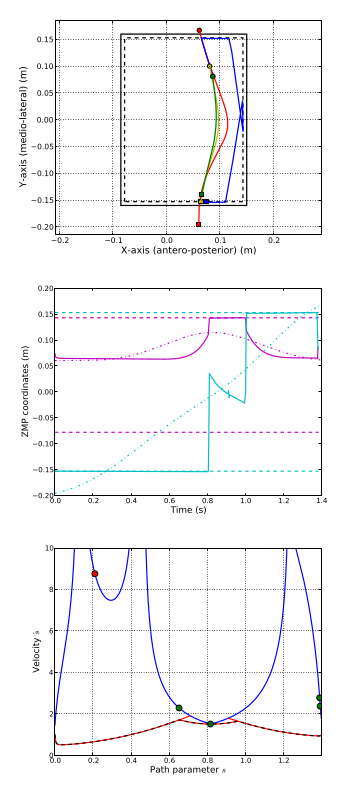
\includegraphics[width=.27\textwidth]{3.png}
  \caption{\textbf{Top:} Trajectories of the ZMP and of the CoM projected on the
ground. The black solid box shows the support area (the robot’s left foot)
and the black dashed box shows the conservative limits for balance. The
trajectory of the projected CoM is in green. The beginnings and endings of
the trajectory were marked respectively by squares and disks. The trajectory
of the ZMP in the original motion (1.40s) is in red. Note that this trajectory
is not contained within the support area: a robot executing this trajectory
would thus stumble. The trajectory of the ZMP in the retimed motion (1.39s)
is in blue. Note that the ZMP trajectory of the retimed motion (blue) is
contained within the conservative limits ensuring thereby the balance. To
achieve the same result, a “scaling down” method – where the velocity
is uniformly reduced – would yield a much slower trajectory, of duration
2.90s (yellow). \textbf{Middle:} X- (magenta) and Y- (cyan) coordinates of the ZMP
trajectories in time. Initial motion in dashed-dotted lines, retimed motion in
plain lines, conservative limits in dashed lines. Note that at any time instant,
at least one of the limits is saturated, which is a necessary condition for
time optimality. \textbf{Bottom:} maximum velocity curve (blue) in the (s, ṡ) plane.
The possible tangent points and “zero-inertia” points are marked in red
and green respectively. The limiting curves are plotted in red and the final
velocity curve is black dashed. For the definition of the terms just used and
not defined here, cf. [13].}
  \label{img3}
\end{figure}

\section*{Acknowledgment}
We would like to thank Dr. R. Diankov for stimulating
discussions and help with OpenRAVE. This work was sup-
ported by “Grants-in-Aid for Scientific Research” for JSPS
fellows and by a JSPS postdoctoral fellowship.

\begin{figure*}[t]
  \centering
  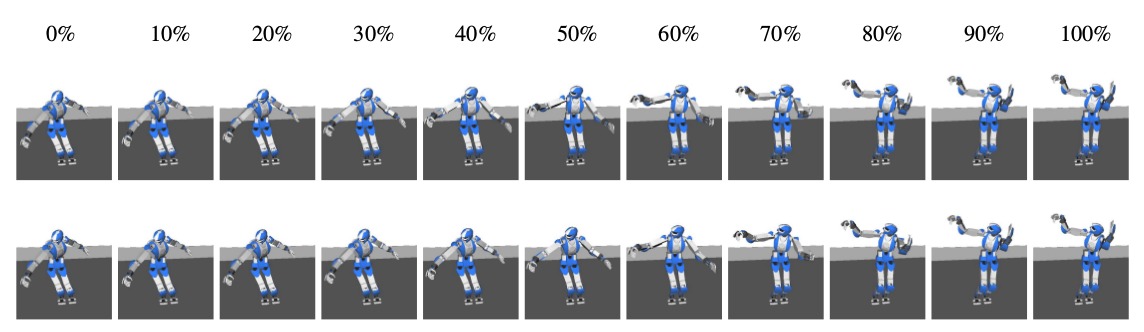
\includegraphics[width=.9\textwidth]{2.png}
  \caption{Snapshots of the whole-body trajectories. Top row: original motion (1.40s). Bottom row: retimed motion (1.39s). Note that the differences
between the two motions are very subtle, yet their balance properties are completely different.}
  \label{img2}
\end{figure*}


\newpage

\begin{thebibliography}{1}


\bibitem{IEEEhowto:kopka}
J.E. Bobrow, S. Dubowsky, and JS Gibson. Time-optimal control of robotic manipulators along specified
paths.\emph{The International Journal of Robotics Research,}, 4(3):3–17, 1985.

\end{thebibliography}
\end{document}
 
